\documentclass{article}
\usepackage[utf8]{inputenc}

\title{Report.5.gaussian.blur.tex}
\author{gw.muraro}
\date{November 1st 2018}

\usepackage{natbib}
\usepackage{graphicx}
\usepackage{pgfplots}
\usepackage{minted}

\begin{document}

\maketitle
\section{Labwork 5}

\subsection{Explain how you implement the Gaussian Blur filter}
    
    The implementation was in several steps :

    \begin{enumerate}     

    \item
     Copy-paste the lab 4 GPU function on the lab 5. We will modify it later, just make it call the new kernel function : 
    \begin{minted}{c}
        gaussianBlur<<<gridSize, blockSize2>>>(devInput, devBlur,
        inputImage->width, inputImage->height, blurDim) ; 
    \end{minted}
    
    \item 
    Begin the implementation of the kernel function. Get the main pixel and do not forget to manage the out-of-bound pixels. Then apply the CPU algorithm adapted to our kernel. For now we use a global blur matrix, it will change. \textbf{This kernel use global memory, we will update it to implement the shared memory.}
    
    \begin{minted}[obeytabs=true,tabsize=2]{c}
    __global__ void gaussianBlur (uchar3 * input, uchar3 * output, 
        int imageWidth, int imageHeight, int blurDim) {

        int blurMatrix[] = {0, 0,  1,  2,   1,  0,  0,  
                     	0, 3,  13, 22,  13, 3,  0,  
                     	1, 13, 59, 97,  59, 13, 1,  
                     	2, 22, 97, 159, 97, 22, 2,  
                     	1, 13, 59, 97,  59, 13, 1,  
                     	0, 3,  13, 22,  13, 3,  0,
                     	0, 0,  1,  2,   1,  0,  0 };
	
	    // getting the pixel location 
	    int tidx = threadIdx.x + blockIdx.x * blockDim.x ;
	    int tidy = threadIdx.y + blockIdx.y * blockDim.y ;
	    int originTid = tidx +  imageWidth *  tidy ;// getting the center pixel 	
	    int relativTid; // this px is nearby the center pixel

	    // if the center pixel is not out of bound 
	    if( tidx >= imageWidth || tidy >= imageHeight) return ;
	
	    /* ALGORITHM IMPLEMENTATION */
	    // sum of the pixel (weight * value) and coeficient 
	    int sum = 0 ;
	    int coef = 0 ;
	
        // Process the 9 pixels 
        for (int i = -(blurDim) ; i < (blurDim) ; i++){
            for (int j = -(blurDim) ; j < (blurDim) ; j++) {
			
            // getting the relative position of our relativPixel in X and Y
            int x = tidx + i ;
            int y = tidy + j ;
			
            // Checking if it is not out of bounds...
            if (x >= imageWidth  || x < 0) continue ;
            if (y >= imageHeight || y < 0) continue ;

            // working on a specific pixel relative to the threaded pixel
            relativTid = imageWidth * y + x ;
			
            // applying the blur on gray pixel 
            unsigned char gray = (input[relativTid].x + 
			                        input[relativTid].y + 
			                        input[relativTid].z) /3;
            int coefficient = blurMatrix[(j+blurDim) * 7 + (i+blurDim)];
            sum  = sum + gray * coefficient ;
            coef += coefficient;
        }
    }
    sum /= coef;
    output[originTid].x = output[originTid].y = output[originTid].z = sum ;
}
    \end{minted}
    
    \item 
    Now we can update it into a \textbf{shared memory kernel}. The algorithm is the same, we will change the blur matrix in order to be a shared variable. For that, we will first pass an array with the blur matrix and adapt our kernel function (blurDim is about the blur intensity, it is by default 3) : 
    \begin{minted}{c}
        // initiate the variable
        int * devWeight ;
        // allocate and copy the array 
        cudaMalloc(&devWeight, sizeof(blurMatrix)); 
        cudaMemcpy(devWeight, blurMatrix, sizeof(blurMatrix), 
        cudaMemcpyHostToDevice);
        // launch the kernel function
        gaussianBlurShared<<<gridSize, blockSize2>>>(
            devInput, 
            devBlur, 
            devWeight, 
            inputImage->width, 
            inputImage->height, 
            blurDim
        ) ; 
    \end{minted}
    
    \item 
    Now we can change our kernel function. The 49 first threads will be mandated to initiate the shared memory array by copying the weight matrix (blurMatrix parameter) : 
    \begin{minted}[obeytabs=true,tabsize=2]{c}
        
        // initiate the blurMatrix variable 
        __shared__ int blurMatrix[49] ;
        // make the 49 firsts threads copy the blurMatrix
        if (threadIdx.x <= 49) {
            blurMatrix[threadIdx.x] = weight[threadIdx.x] ;
        }
        // wait for threads to synchronize
        __syncthreads() ;
    \end{minted}
    \end{enumerate}
\subsection{Results ! (finaly)}
By using timers and a little bash script, we can see these results with different block number in 2D (3$^{rd}$ argument of the labwork program) :
    \begin{verbatim}
    ==== labwork 5 ../data/eiffel.jpg 4 
    USTH ICT Master 2018, Advanced Programming for HPC.
    Warming up...
    Starting labwork 5
    labwork 5 ellapsed 1737.4ms (CPU)
    labwork 5 ellapsed 48.3ms (GPU global memory)
    labwork 5 ellapsed 33.6ms (GPU shared memory)
    
    ==== labwork 5 ../data/eiffel.jpg 16
    USTH ICT Master 2018, Advanced Programming for HPC.
    Warming up...
    Starting labwork 5
    labwork 5 ellapsed 1714.0ms (CPU)
    labwork 5 ellapsed 44.5ms (GPU global memory)
    labwork 5 ellapsed 28.9ms (GPU shared memory)
    
    ==== labwork 5 ../data/eiffel.jpg 32
    USTH ICT Master 2018, Advanced Programming for HPC.
    Warming up...
    Starting labwork 5
    labwork 5 ellapsed 1717.4ms (CPU)
    labwork 5 ellapsed 40.9ms (GPU global memory)
    labwork 5 ellapsed 24.8ms (GPU shared memory)



    \end{verbatim}

\subsection{Plot a graph}
   %%plot
    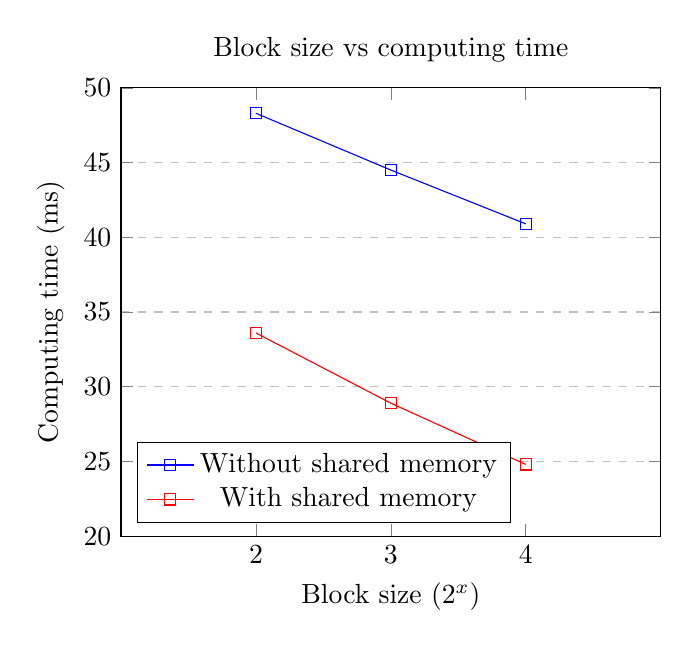
\begin{tikzpicture}
        \centering
        %%define axes
        \begin{axis}[
            title={Block size vs computing time},
            xlabel={Block size ($2^x$)},
            ylabel={Computing time (ms)},
            xmin=1, xmax=5,
            ymin=20, ymax=50,
            xtick={2,3,4},
            ytick={20, 25, 30, 35, 40, 45, 50},
            legend pos=south west,
            ymajorgrids=true,
            grid style=dashed,
        ]
        %% data filing
        \addplot[
            color=blue,
            mark=square,
            ]
            coordinates { %% Remind : axis X = 2^x
                (2,48.3)(3,44.5)(4,40.9)
            };
        \addplot[
            color=red,
            mark=square,
            ]
            coordinates { %% Remind : axis X = 2^x
                (2,33.6)(3,28.9)(4,24.8)
            };
        
        \legend{Without shared memory,With shared memory}
        \end{axis}
    \end{tikzpicture}
    \newline


\end{document}

